\label{sec:fuzzing}
After the assembly inspection has performed the static analysis and flagged programs with potential timing vulnerabilities, OptiFuzz tries and confirm their presence. 
For this, we have created a fuzzer.
In this section, we explain the process of compiling, running, and timing the programs.
This process is illustrated in Figure \ref{fig:fuzzer-pipeline}.
%First, the fuzzer compiles the program with the specified compiler and optimization level flags.
%Then, the fuzzer runs the program with random inputs and measures the execution time.
The process goes as follows: 
First, the fuzzer itself is compiled into object files (simplified to a single file in Figure \ref{fig:fuzzer-pipeline}) that are not yet linked. 
This compilation happens once.
Each of the programs flagged by the assembly inspection is then compiled with the specified compiler and optimization flags.
After a program has been compiled it is linked with the fuzzer and is run.

\begin{figure}[H]
    \centering
    \tikzstyle{box-nb} = [rectangle, minimum width=1.3cm, minimum height=0.3cm, text centered]
\tikzstyle{box} = [rectangle, minimum width=2.2cm, minimum height=0.8cm, text centered, draw=black]
\tikzstyle{arrow} = [thick,->,>=stealth]

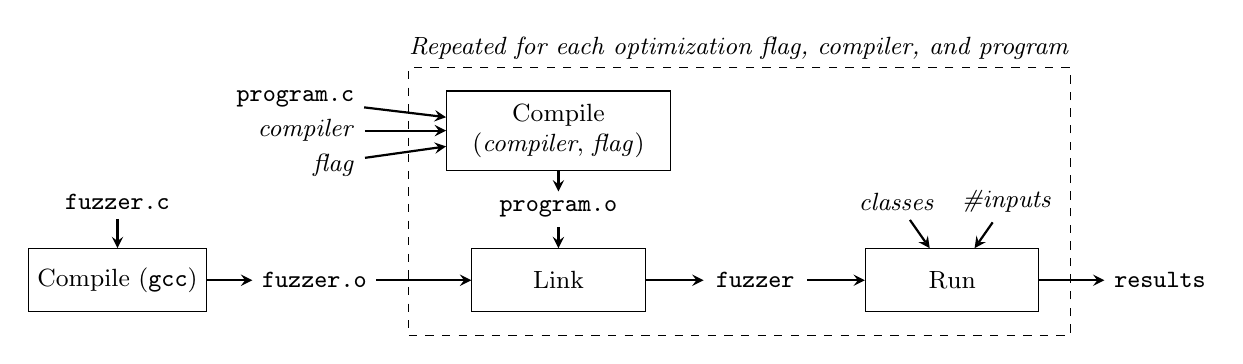
\begin{tikzpicture}
  \node (comp_prog) [box] {\small \begin{tabular}{c} Compile \\ (\textit{compiler}, \textit{flag}) \end{tabular} };
  \node (programo) [box-nb, below of=comp_prog] {\small \texttt{program.o}};
  \node (link) [box, below of=programo, yshift=0.1cm] {\small Link};
  \node (fuzzero) [box-nb, left of=link, xshift=-2.1cm] {\small \texttt{fuzzer.o}};
  \node (comp_fuzz) [box, left of=fuzzero, xshift=-1.5cm] {\small Compile (\texttt{gcc})};
  \node (fuzzerc) [box-nb, above of=comp_fuzz] {\small \texttt{fuzzer.c}};
  \node (fuzzer) [box-nb, right of=link, xshift=1.5cm] {\small \texttt{fuzzer}};
  \node (run) [box, right of=fuzzer, xshift=1.5cm] {\small Run};
  \node (classes) [box-nb, above of=run, xshift=-0.7cm] {\small \textit{classes}};
  \node (inputs) [box-nb, above of=run, xshift=0.7cm] {\small \textit{\#inputs}};
  \node (results) [box-nb, right of=run, xshift=1.64cm] {\small \texttt{results}};
  \node (programc) [box-nb, left of=comp_prog, yshift=0.4cm, xshift=-2.34cm] {\small \texttt{program.c}};
  \node (compiler) [box-nb, left of=comp_prog, xshift=-2.2cm] {\small \textit{compiler}};
  \node (flag) [box-nb, left of=comp_prog, yshift=-0.4cm, xshift=-2.13cm, yshift=-0.04cm] {\small \textit{\quad\ \ flag}};
  \node (repeat) [rectangle, draw=black, dashed, minimum height=3.4cm, minimum width=8.4cm, yshift=-0.9cm, xshift=2.3cm] {};
  \node (repeat-text) [box-nb, above of=repeat, yshift=0.95cm] {\small \textit{Repeated for each optimization flag, compiler, and program }};
  
  \draw [arrow] (fuzzerc) -- (comp_fuzz);
  \draw [arrow] (comp_fuzz) -- (fuzzero);
  \draw [arrow] (comp_prog) -- (programo);
  \draw [arrow] (programo) -- (link);
  \draw [arrow] (fuzzero) -- (link);
  \draw [arrow] (link) -- (fuzzer);
  \draw [arrow] (fuzzer) -- (run);
  \draw [arrow] (run) -- (results);
  \draw [arrow] (programc)-- (comp_prog);
  \draw [arrow] (compiler) -- (comp_prog);
  \draw [arrow] (flag) -- (comp_prog);
  \draw [arrow] (classes) -- (run);
  \draw [arrow] (inputs) -- (run);
\end{tikzpicture}
    \caption{Illustration of the process of compiling and fuzzing programs. The fuzzer is compiled once, after which the process in the dashed box is repeated with different programs, compilers, and flags emitting results.}
    \label{fig:fuzzer-pipeline}
\end{figure}

When running the fuzzer, it generates inputs according to 'input classes' dictating the nature of the generated values.
Each input is independently generated according to a uniformly random class among the supplied ones.
The fuzzer then executes the linked program for each of the inputs and measures their execution time.

We use different input classes for generating inputs for the program. 
This is done to try and capture deviating execution times that only take place for a small sample of the values.
If we only used uniformly random 64-bit numbers it would be very unlikely that we would identify such a vulnerability.
Hence, the need for input classes.
As mentioned in Section \ref{sec:code-generation}, for each program, there are an $x$ and a $y$ value passed as arguments. 
Each input classes generate such a pair of inputs according to the following list.
\begin{itemize}
    \setlength\itemsep{-0.6em}
    \item \texttt{UNIFORM}: $x$ and $y$ are uniformly random 64-bit numbers.
    \item \texttt{EQUAL}:  $x$ and $y$ are the same uniformly random 64-bit number.
    \item \texttt{MAX64}: Either $x$ or $y$ is a random 64-bit number, the other is uniformly random.
    \item \texttt{XZERO}: $x$ is 0, $y$ is a uniformly random number.
    \item \texttt{YZERO}: $y$ is 0, $x$ is a uniformly random number.
    \item \texttt{XLTY}: Two uniformly random numbers are generated, $x$ is set to the smaller, $y$ to the larger.
    \item \texttt{YLTX}: Two uniformly random numbers are generated, $y$ is set to the smaller, $x$ to the larger.
    \item \texttt{SMALL}: $x$ and $y$ are uniformly random 8-bit numbers (the upper 56 bits are set to 0).
    \item \texttt{FIXED}: $x$ and $y$ have the same fixed number $0x12345678$ (used for Welsh's t-test).
\end{itemize}
These classes have been chosen based on observations of types of values commonly used in conditions in the emitted assembly code.

Precise measurements of a program's execution time are not trivial to perform. 
Measurements can be influenced by several things including context switches, interrupts, out-of-order execution, varying CPU clock speed, and congestion. 
For timing, we use the Time Stamp Counter (\texttt{TSC}) as our source.
The \texttt{TSC} is a high-resolution counter that (on newer machines) increases at a fixed rate independent of processor frequency and is the most efficient wall clock resource according to \citep[b]{intel-reference}.
Alternatives like \texttt{HPET} with higher resolutions exist but read the time from a platform resource instead of a register, making it much slower \citep[b]{intel-reference}.
This method is the one suggested by \citep{intel-benchmark-code-execution} and is the one used in the DudeCT black-box testing tool by \citep{dudect}.
This approach also allowed us to avoid the timings being skewed by the CPU performing out-of-order execution.
Out-of-order executions could lead to the instructions being reordered resulting in not reading the \texttt{TSC} (with the \texttt{RDTSC}(\texttt{P}) instruction) at the correct time. 
This is mitigated by utilizing the non-privileged \texttt{CPUID} instructions serializing capabilities that ensure that memory transactions for previous instructions are completed before the next instruction is executed \citep[a]{intel-reference}.
Using \texttt{CPUID} and \texttt{RDTSCP} allows us to enclose the program call between our time measures using \texttt{RDTSC}(\texttt{P}) as wanted.

\subsubsection{Limitations}
We consider the fuzzer successful when it consistently measures a clear difference in the execution time of a program concerning its input classes.
This indicates that the program is vulnerable with high probability.
However, it is not safe to assume that the program is constant time when the fuzzer is not able to measure variable time.
Since the fuzzer is conservative, it under-approximates what programs are vulnerable to timing attacks.
Hence, a limitation is that the input classes used are not necessarily able to capture an event causing variable-time behavior of a program.

Another limitation is that the timings produced are still prone to some noise.
Specifically, when running this in user-land the fuzzer could be influenced by interrupts and preemption (OS forces context switches). 
To combat these, one is required to run the code in kernel space as suggested by \citep{intel-benchmark-code-execution}.
It is however possible to mitigate some of this noise by running the fuzzer with higher priority. 
